\documentclass{article}

\usepackage{graphicx}
\usepackage{verbatim}

\author{Mohammad Afroz Alam}
\date{}
\title{CV Assignment 3 Readme}
\begin{document}

\section{Time Taken}
\begin{itemize}
\item Time taken for conv1 = 0.000958919525146 secs
\item Time taken for conv2 = 0.00978302955627 secs
\item Time taken for conv3 = 0.00294518470764 secs
\item Time taken for conv4 = 0.00292491912842 secs
\item Time taken for conv5 = 0.0381109714508 secs
\item Time taken for fc1 = 0.000120878219604 secs
\item Time taken for fc2 = 0.000124216079712 secs
\end{itemize}

\section{Number of Parameters}
\begin{itemize}
\item Conv 1 : 155
\item Conv 2 : 2416
\item Fc 1 : 48120
\item Fc 2 : 10164
\item Fc 3 : 850
\end{itemize}

\section{t-SNE plots}
\begin{figure}[h]
  \centering
  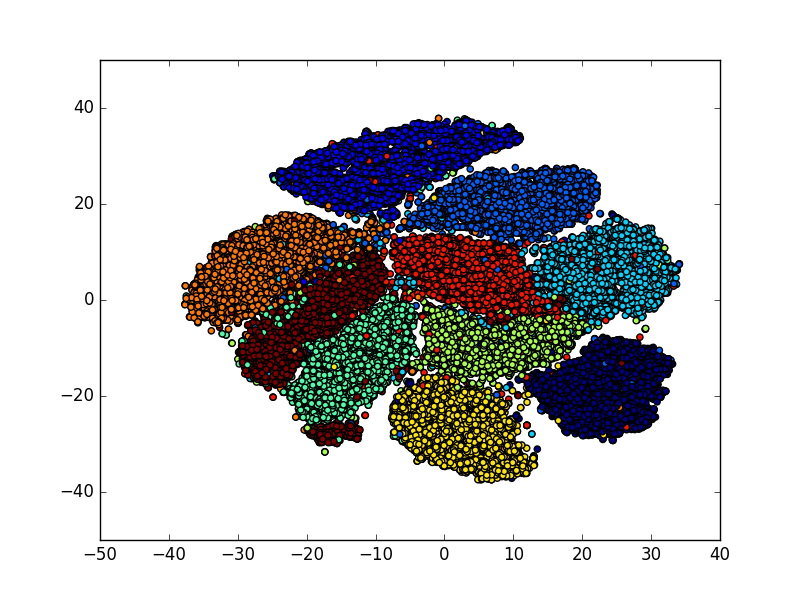
\includegraphics[width=0.7\textwidth]{keras_lenet/scatter_basic.png}
  \caption{Without 84 dimensional features}
  \label{fig:basic}
\end{figure}

\begin{figure}[h]
  \centering
  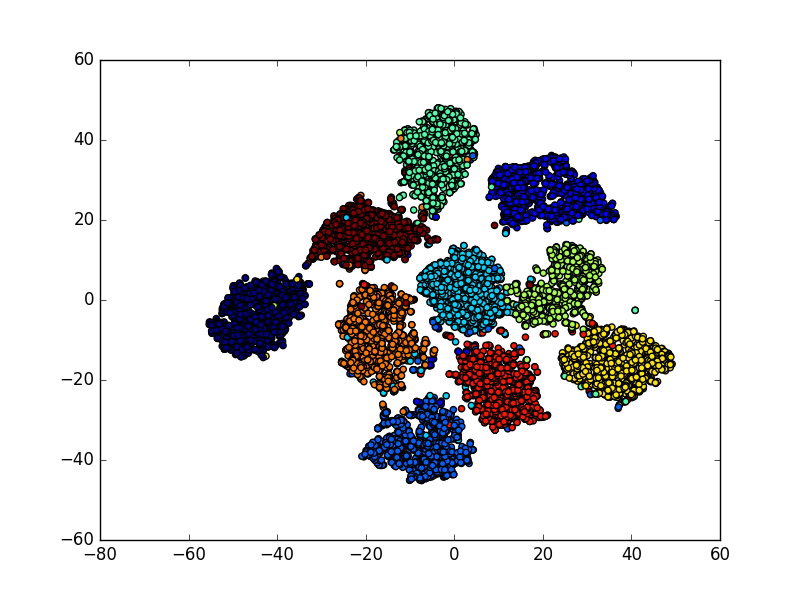
\includegraphics[width=0.7\textwidth]{keras_lenet/scatter_encoding.png}
  \caption{With 84 dimensional features}
\end{figure}

\section{Training and Validation Losses}

\begin{figure}[h]
  \centering
  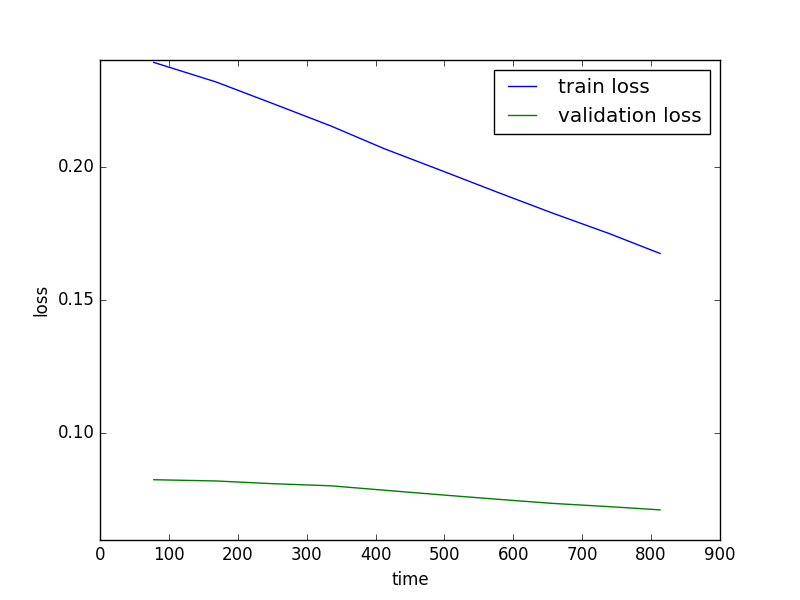
\includegraphics[width=0.7\textwidth]{keras_lenet/loss32.png}
  \caption{Train and Validation loss for batch size 32}
\end{figure}

\begin{figure}[h]
  \centering
  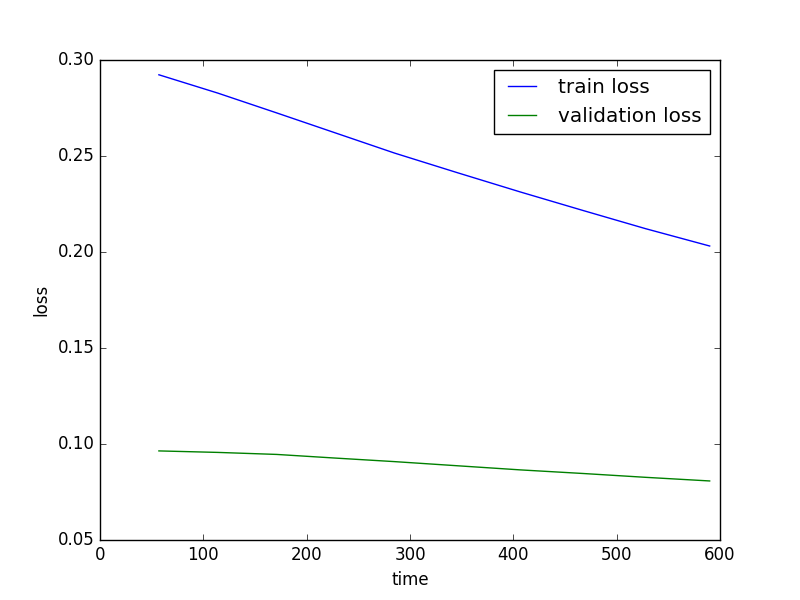
\includegraphics[width=0.7\textwidth]{keras_lenet/loss64.png}
  \caption{Train and Validation loss for batch size 64}
\end{figure}

\begin{figure}[h]
  \centering
  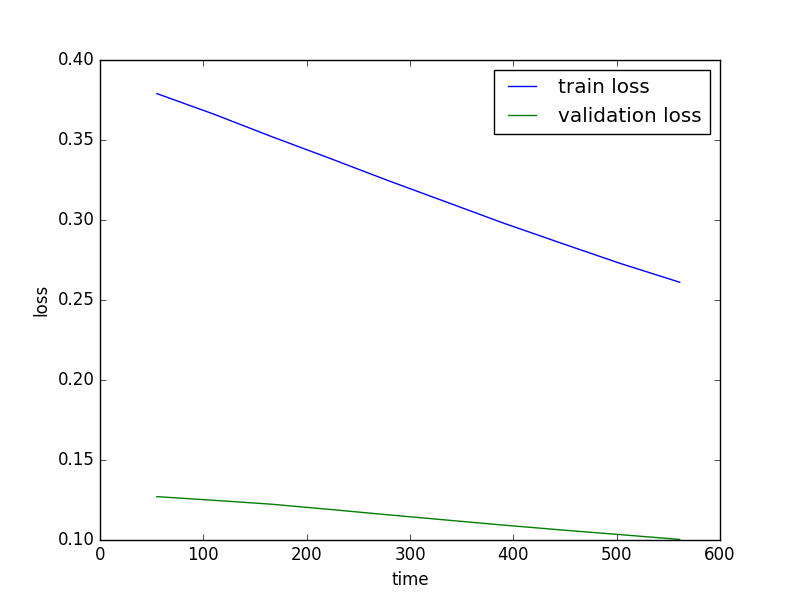
\includegraphics[width=0.7\textwidth]{keras_lenet/loss128.png}
  \caption{Train and Validation loss for batch size 128}
\end{figure}

\begin{figure}[h]
  \centering
  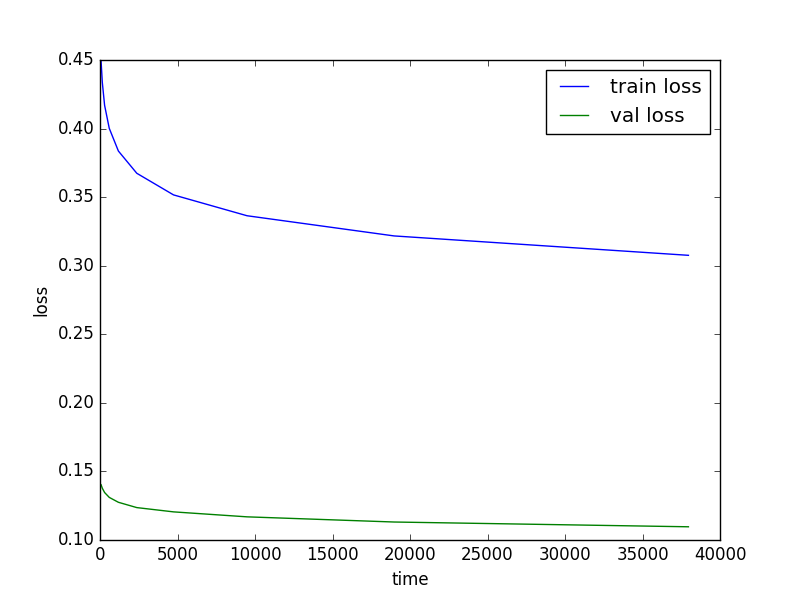
\includegraphics[width=0.7\textwidth]{keras_lenet/loss200.png}
  \caption{Train and Validation loss for batch size 200}
\end{figure}

\begin{figure}[h]
  \centering
  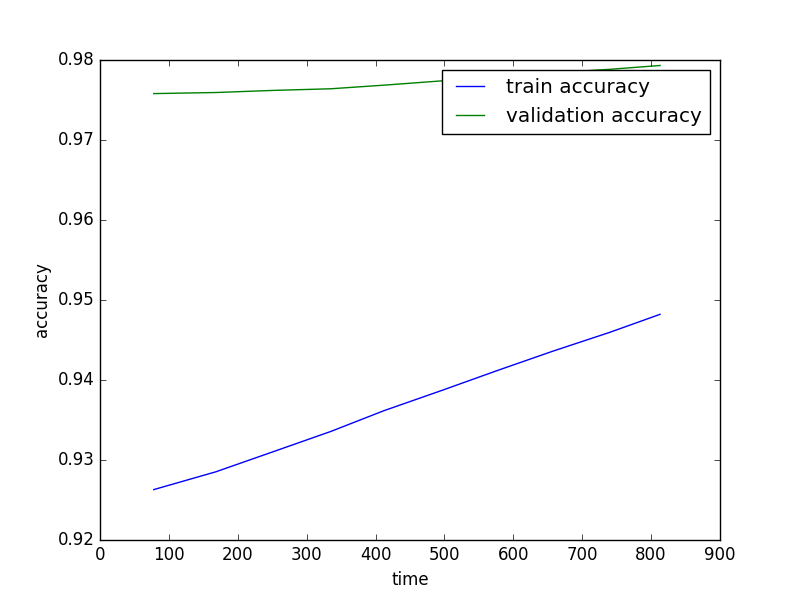
\includegraphics[width=0.7\textwidth]{keras_lenet/accuracy32.png}
  \caption{Train and Validation accuracy for batch size 32}
\end{figure}

\begin{figure}[h]
  \centering
  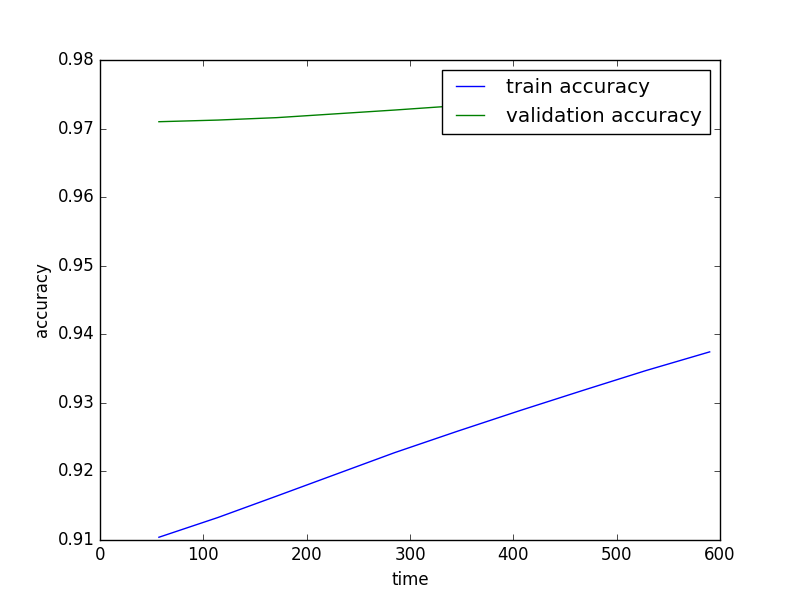
\includegraphics[width=0.7\textwidth]{keras_lenet/accuracy64.png}
  \caption{Train and Validation accuracy for batch size 64}
\end{figure}

\begin{figure}[h]
  \centering
  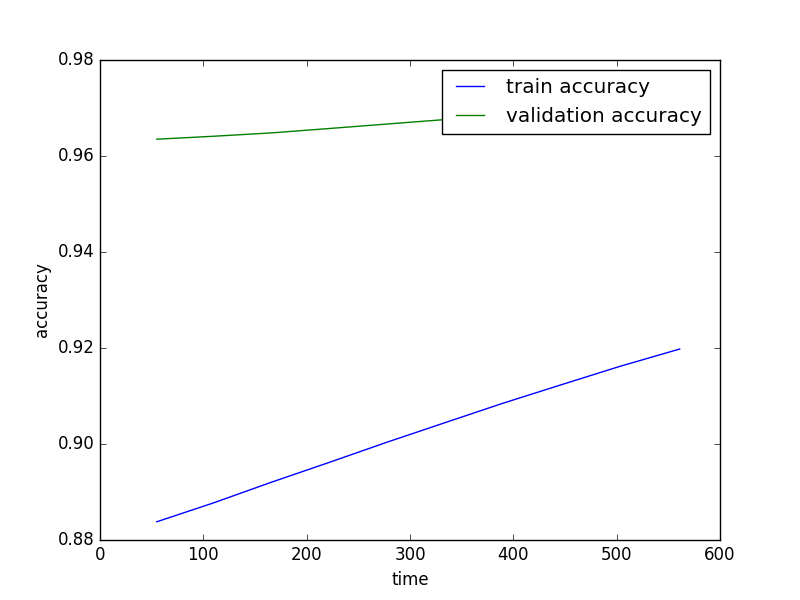
\includegraphics[width=0.7\textwidth]{keras_lenet/accuracy128.png}
  \caption{Train and Validation accuracy for batch size 128}
\end{figure}

\begin{figure}[h]
  \centering
  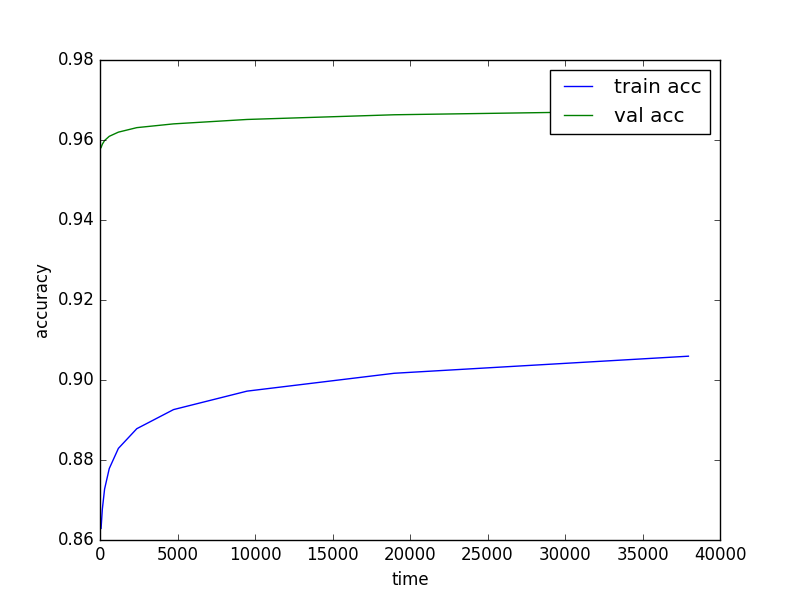
\includegraphics[width=0.7\textwidth]{keras_lenet/accuracy200.png}
  \caption{Train and Validation accuracy for batch size 200}
\end{figure}



\end{document}
